% Task C26
% Source volume: lower
% Physical scan pages: 383--397
% Printed book pages: 371--385
% Transcribe only source content; omit running headers, footers, and printed page numbers.
\chapter{场论初步}

% BEGIN TRANSCRIPTION

场本来是物理学的研究对象，如温度场、电磁场、重力场等。这些场除了有各自不同的物理性质之外，表现在数量关系上可分为数量场与向量场。

本章介绍场论的初步数学知识。在 §26.1 引入散度和旋度的概念，然后将梯度、散度、旋度与 Green 公式、Gauss 公式、Stokes 公式融合在一起，展现多元积分丰富多彩的一面。在 §26.2 中介绍 Laplace 算子和有关调和函数的一些知识。最后一节是学习要点和两组参考题。

\section{散度和旋度}

\subsection{散度}

设 $D$ 是 $\RR^3$ 中的一个区域，
\[
  \vect{a}(x,y,z)=P(x,y,z)\vect{i}+Q(x,y,z)\vect{j}+R(x,y,z)\vect{k}
\]
是定义在 $D$ 上的向量值函数，称 $\vect{a}$ 是定义在 $D$ 上的一个\textbf{向量场}。又设 $P,Q,R$ 有连续的偏导数，记
\[
  \operatorname{div}\vect{a}
  =\frac{\partial P}{\partial x}+\frac{\partial Q}{\partial y}+\frac{\partial R}{\partial z},
\]
称之为向量场 $\vect{a}$ 的散度，它是一个数量，有时也记为 $\nabla\cdot\vect{a}$。注意与一个三元函数 $f$ 的梯度 $\nabla f$ 的区别（见 21.2.2 小节）。

类似地在 $\RR^2$ 中，若 $\vect{a}=P(x,y)\vect{i}+Q(x,y)\vect{j}$，则
\[
  \operatorname{div}\vect{a}=\frac{\partial P}{\partial x}+\frac{\partial Q}{\partial y}.
\]

利用散度的记号，可以将 Gauss 公式 (25.5)，(25.6) 写为
\begin{equation}
  \iiint_D \operatorname{div}\vect{a}\,\dd x\,\dd y\,\dd z
  =\oiint_{\partial D} P\,\dd y\,\dd z+Q\,\dd z\,\dd x+R\,\dd x\,\dd y,
  \tag{26.1}
  \label{eq:26.1}
\end{equation}
\begin{equation}
  \iiint_D \operatorname{div}\vect{a}\,\dd x\,\dd y\,\dd z
  =\oiint_{\partial D}\vect{a}\cdot\vect{n}\,\dd S,
  \tag{26.2}
  \label{eq:26.2}
\end{equation}
其中 $\vect{a}=(P,Q,R)$，$\vect{n}$ 是 $\partial D$ 上的单位外法向量。而将 Green 公式 (24.9)，(24.10) 写为
\begin{equation}
  \iint_D \operatorname{div}\vect{a}\,\dd x\,\dd y
  =\oint_{\partial D}-Q\,\dd x+P\,\dd y,
  \tag{26.3}
  \label{eq:26.3}
\end{equation}
\begin{equation}
  \iint_D \operatorname{div}\vect{a}\,\dd x\,\dd y
  =\oint_{\partial D}\vect{a}\cdot\vect{n}\,\dd s.
  \tag{26.4}
  \label{eq:26.4}
\end{equation}
又可将公式 (26.2) 与 (26.4) 统一写为
\begin{equation}
  \int_D \operatorname{div}\vect{a}\,\dd V
  =\int_{\partial D}\vect{a}\cdot\vect{n}\,\dd S.
  \tag{26.5}
  \label{eq:26.5}
\end{equation}
上述公式称为\textbf{散度定理}，它对任意维数都是成立的。

$n=1$ 时，一元函数 $f(x)$ 的散度是 $f'(x)$，$\dd V=\dd x$，在区间的左端点 $n=-1$，在区间的右端点 $n=1$，在区间端点的点积分理解为被积函数在该点的值，则 (26.5) 就是 Newton--Leibniz 公式。

$n=2$ 时 (26.5) 就是 Green 公式，$\dd V$ 为面积元。

$n=3$ 时 (26.5) 就是 Gauss 公式，$\dd V$ 是体积元，$\vect{n}$ 是 $\partial D$ 上的单位外法向量。

\begin{xexample}[26.1.1]
证明重积分的分部积分公式
\[
  \iiint_\Omega u\frac{\partial v}{\partial x}\,\dd x\,\dd y\,\dd z
  =\oiint_\Sigma uv\,\dd y\,\dd z
  -\iiint_\Omega v\frac{\partial u}{\partial x}\,\dd x\,\dd y\,\dd z,
\]
其中 $\Sigma$ 是 $\Omega$ 的边界，分片光滑，取外侧；$u,v$ 在 $\overline\Omega$ 上连续可微。
\end{xexample}
\begin{xproof}
在 (26.1) 中令 $\vect{a}=(uv,0,0)$，则
\[
  \iiint_\Omega\left(u\frac{\partial v}{\partial x}+v\frac{\partial u}{\partial x}\right)\,\dd x\,\dd y\,\dd z
  =\oiint_\Sigma uv\,\dd y\,\dd z.
\]
\end{xproof}
\begin{xremark}
令 $v=1$，则有
\[
  \iiint_\Omega\frac{\partial u}{\partial x}\,\dd x\,\dd y\,\dd z
  =\oiint_\Sigma u\,\dd y\,\dd z.
\]
\end{xremark}

\subsection{旋度}

设 $\vect{a}=P\vect{i}+Q\vect{j}+R\vect{k}$ 是定义在区域 $D$ 上的向量场，又设 $P,Q,R$ 在 $D$ 上有连续偏导数。记
\[
  \operatorname{curl}\vect{a}
  =\begin{vmatrix}
    \vect{i}&\vect{j}&\vect{k}\\
    \dfrac{\partial}{\partial x}&\dfrac{\partial}{\partial y}&\dfrac{\partial}{\partial z}\\
    P&Q&R
  \end{vmatrix}
\]
\[
  =\left(\frac{\partial R}{\partial y}-\frac{\partial Q}{\partial z}\right)\vect{i}
  +\left(\frac{\partial P}{\partial z}-\frac{\partial R}{\partial x}\right)\vect{j}
  +\left(\frac{\partial Q}{\partial x}-\frac{\partial P}{\partial y}\right)\vect{k},
\]
称之为向量场 $\vect{a}$ 的旋度。它是一个向量，有时也记为 $\nabla\times\vect{a}$。利用旋度的记号，可将 Stokes 公式 (25.13) 写为
\[
  \iint_D \operatorname{curl}\vect{a}\cdot\vect{n}\,\dd S
  =\oint_{\partial D}\vect{a}\cdot\vect{\tau}\,\dd s,
\]
其中 $D$ 是空间曲面，$\partial D$ 是它的边界，$\vect{a}=(P,Q,R)$，等式左端的 $\vect{n}$ 为 $D$ 的单位外法向量，等式右端的 $\vect{\tau}$ 是 $\partial D$ 的切向量。它们两者的方向服从右手系法则。

在下面需要星形区域的概念。

\begin{xdefinition}
设 $M$ 是区域 $G$ 内一点，称 $G$ 是关于 $M$ 的星形区域，如果对任意一点 $P\in G$，都有 $P$ 与 $M$ 之间的直线段 $PM\subset G$。
\end{xdefinition}

\begin{xexample}[26.1.2]
设 $G$ 是 $\RR^3$ 中关于其内一点 $M$ 的星形区域。$\vect{F}=(P,Q,R)$ 是 $G$ 上的光滑向量场，且 $\operatorname{div}\vect{F}=0$。证明：存在 $G$ 上的光滑向量场 $\vect{A}$，使得
\[
  \vect{F}=\operatorname{curl}\vect{A}.
\]
\end{xexample}
\begin{xproof}
不妨设 $M$ 为原点。由于 $G$ 关于原点为星形区域，于是对任何 $(x,y,z)\in G$，有
\begin{align}
  P(x,y,z)
  &=\int_0^1\frac{\partial}{\partial t}\bigl[t^2P(tx,ty,tz)\bigr]\,\dd t\notag\\
  &=2\int_0^1 tP(tx,ty,tz)\,\dd t
  +\int_0^1 t^2\frac{\partial}{\partial t}P(tx,ty,tz)\,\dd t.
  \tag{26.6}
  \label{eq:26.6}
\end{align}
由已知条件有
\[
  \frac{\partial P}{\partial x}
  =-\frac{\partial Q}{\partial y}-\frac{\partial R}{\partial z},
\]
将它代入 (26.6) 中，则
\begin{align*}
  P(x,y,z)
  ={}&2\int_0^1 tP(tx,ty,tz)\,\dd t\\
  &-\int_0^1 t^2x\left[\frac{\partial Q}{\partial y}(tx,ty,tz)+\frac{\partial R}{\partial z}(tx,ty,tz)\right]\,\dd t\\
  &+\int_0^1 t^2y\frac{\partial P}{\partial y}(tx,ty,tz)\,\dd t
  +\int_0^1 t^2z\frac{\partial P}{\partial z}(tx,ty,tz)\,\dd t\\
  ={}&\frac{\partial}{\partial y}\left[y\int_0^1tP(tx,ty,tz)\,\dd t-x\int_0^1tQ(tx,ty,tz)\,\dd t\right]\\
  &-\frac{\partial}{\partial z}\left[x\int_0^1tR(tx,ty,tz)\,\dd t-z\int_0^1tP(tx,ty,tz)\,\dd t\right].
\end{align*}
记
\begin{align*}
  A_1(x,y,z)&=z\int_0^1tQ(tx,ty,tz)\,\dd t-y\int_0^1tR(tx,ty,tz)\,\dd t,\\
  A_2(x,y,z)&=x\int_0^1tR(tx,ty,tz)\,\dd t-z\int_0^1tP(tx,ty,tz)\,\dd t,\\
  A_3(x,y,z)&=y\int_0^1tP(tx,ty,tz)\,\dd t-x\int_0^1tQ(tx,ty,tz)\,\dd t,
\end{align*}
则
\[
  P(x,y,z)=\frac{\partial A_3}{\partial y}-\frac{\partial A_2}{\partial z}.
\]
同理可证
\[
  Q(x,y,z)=\frac{\partial A_1}{\partial z}-\frac{\partial A_3}{\partial x},
  \qquad
  R(x,y,z)=\frac{\partial A_2}{\partial x}-\frac{\partial A_1}{\partial y}.
\]
令 $\vect{A}=(A_1,A_2,A_3)$，则
\[
  \vect{F}=\operatorname{curl}\vect{A}.
\]
\end{xproof}

\subsection{\texorpdfstring{Hamilton 算子 $\nabla$}{Hamilton 算子 ∇}}

$\nabla$ 是一个算子符号，称为 Hamilton（哈密顿）算子。它的定义是
\[
  \nabla=\vect{i}\frac{\partial}{\partial x}
  +\vect{j}\frac{\partial}{\partial y}
  +\vect{k}\frac{\partial}{\partial z}.
\]
其具体含义如下：设 $f$ 是一个可微函数，则
\[
  \nabla f=\vect{i}\frac{\partial f}{\partial x}
  +\vect{j}\frac{\partial f}{\partial y}
  +\vect{k}\frac{\partial f}{\partial z},
\]
即
\[
  \nabla f=\operatorname{grad}f\qquad(f\text{ 的梯度}).
\]
设 $\vect{a}$ 是一个向量场，$\vect{a}=P\vect{i}+Q\vect{j}+R\vect{k}$，则
\[
  \nabla\cdot\vect{a}=\operatorname{div}\vect{a},
  \qquad
  \nabla\times\vect{a}=\operatorname{curl}\vect{a}.
\]
因此，我们也常用 $\nabla\cdot\vect{a}$ 和 $\nabla\times\vect{a}$ 分别表示 $\vect{a}$ 的散度与旋度。直接运算可以证明下列关系式（其中 $\alpha,\beta$ 为常数，$f,g$ 为数量函数，$\vect{a},\vect{b}$ 为向量函数）：
\begin{align}
  \nabla(\alpha f+\beta g)&=\alpha\nabla f+\beta\nabla g, \tag{26.7}\label{eq:26.7}\\
  \nabla\cdot(\alpha\vect{a}+\beta\vect{b})&=\alpha\nabla\cdot\vect{a}+\beta\nabla\cdot\vect{b}, \tag{26.8}\label{eq:26.8}\\
  \nabla\times(\alpha\vect{a}+\beta\vect{b})&=\alpha\nabla\times\vect{a}+\beta\nabla\times\vect{b}, \tag{26.9}\label{eq:26.9}\\
  \nabla(fg)&=(\nabla f)g+f(\nabla g), \tag{26.10}\label{eq:26.10}\\
  \nabla\cdot(f\vect{a})&=f(\nabla\cdot\vect{a})+(\nabla f)\cdot\vect{a}, \tag{26.11}\label{eq:26.11}\\
  \nabla\times(f\vect{a})&=f(\nabla\times\vect{a})+(\nabla f)\times\vect{a}, \tag{26.12}\label{eq:26.12}\\
  \nabla\cdot(\nabla\times\vect{a})&=0\qquad(\text{即任一向量函数的旋度的散度为零}), \tag{26.13}\label{eq:26.13}\\
  \nabla\times(\nabla f)&=0\qquad(\text{即任一数量函数的梯度的旋度为零向量}). \tag{26.14}\label{eq:26.14}
\end{align}

\begin{xexample}[26.1.3]
$\vect{A},\vect{B}$ 为可微的向量函数，则
\[
  \nabla\cdot(\vect{A}\times\vect{B})
  =\vect{B}\cdot(\nabla\times\vect{A})-\vect{A}\cdot(\nabla\times\vect{B}).
\]
\end{xexample}
\begin{xproof}
设 $\vect{A}=(a_1,a_2,a_3)$，$\vect{B}=(b_1,b_2,b_3)$，则有
\[
  \vect{A}\times\vect{B}
  =\begin{vmatrix}
    \vect{i}&\vect{j}&\vect{k}\\
    a_1&a_2&a_3\\
    b_1&b_2&b_3
  \end{vmatrix}.
\]
于是
\begin{align*}
  \nabla\cdot(\vect{A}\times\vect{B})
  ={}&\frac{\partial}{\partial x}\begin{vmatrix}a_2&a_3\\b_2&b_3\end{vmatrix}
  -\frac{\partial}{\partial y}\begin{vmatrix}a_1&a_3\\b_1&b_3\end{vmatrix}
  +\frac{\partial}{\partial z}\begin{vmatrix}a_1&a_2\\b_1&b_2\end{vmatrix}\\
  ={}&\begin{vmatrix}\partial_xa_2&\partial_xa_3\\b_2&b_3\end{vmatrix}
  -\begin{vmatrix}\partial_ya_1&\partial_ya_3\\b_1&b_3\end{vmatrix}
  +\begin{vmatrix}\partial_za_1&\partial_za_2\\b_1&b_2\end{vmatrix}\\
  &+\begin{vmatrix}a_2&a_3\\\partial_xb_2&\partial_xb_3\end{vmatrix}
  -\begin{vmatrix}a_1&a_3\\\partial_yb_1&\partial_yb_3\end{vmatrix}
  +\begin{vmatrix}a_1&a_2\\\partial_zb_1&\partial_zb_2\end{vmatrix}\\
  ={}&I_1+I_2,
\end{align*}
其中 $I_1$ 为前三项，$I_2$ 为后三项。经计算验证有
\[
  I_1=b_1(\partial_ya_3-\partial_za_2)+b_2(\partial_za_1-\partial_xa_3)+b_3(\partial_xa_2-\partial_ya_1)
  =\vect{B}\cdot(\nabla\times\vect{A}),
\]
同理可证
\[
  I_2=-\vect{A}\cdot(\nabla\times\vect{B}).
\]
\end{xproof}

\begin{xexample}[26.1.4]
设 $u(x,y,z)$ 在 $\overline{B_R(M_0)}$ 上二阶连续可微，其中 $M_0=(x_0,y_0,z_0)$，$B_R(M_0)$ 是以 $M_0$ 为心、以 $R$ 为半径的球。对于 $0<\rho\le R$，如果都有
\[
  \oiint_{\partial B_\rho(M_0)}\frac{\partial u}{\partial n}(x,y,z)\,\dd S=0,
\]
其中 $\partial B_\rho(M_0)$ 是以 $M_0$ 为心、以 $\rho$ 为半径的球面，$\vect{n}$ 是球面上的单位外法向量，则
\[
  u(M_0)=\frac{1}{4\pi R^2}\oiint_{\partial B_R(M_0)}u(x,y,z)\,\dd S.
\]
即球心的值等于球面上的积分平均值。
\end{xexample}
\begin{xproof}
令
\[
  x=x_0+\rho\sin\varphi\cos\theta,
  \qquad y=y_0+\rho\sin\varphi\sin\theta,
  \qquad z=z_0+\rho\cos\varphi,
\]
\[
  0\le\theta\le2\pi,
  \qquad 0\le\varphi\le\pi.
\]
则在 $\partial B_\rho(M_0)$ 上有
\begin{align*}
  \frac{\partial u}{\partial n}(x,y,z)
  &=\nabla u\cdot\vect{n}\\
  &=\frac{\dd u}{\dd\rho}(x_0+\rho\sin\varphi\cos\theta,
    y_0+\rho\sin\varphi\sin\theta,z_0+\rho\cos\varphi)\\
  &=\frac{\dd u}{\dd\rho}(M_0+\rho\vect{n}).
\end{align*}
于是
\begin{align*}
  0
  &=\oiint_{\partial B_\rho(M_0)}\frac{\partial u}{\partial n}(x,y,z)\,\dd S\\
  &=\rho^2\oiint_{\partial B_1(0)}\frac{\dd u}{\dd\rho}(M_0+\rho\vect{n})\,\dd S_1\qquad(\text{由 }(25.28))\\
  &=\rho^2\frac{\dd}{\dd\rho}\oiint_{\partial B_1(0)}u(M_0+\rho\vect{n})\,\dd S_1.
\end{align*}
由此可得到
\[
  \frac{\dd}{\dd\rho}\oiint_{\partial B_1(0)}u(M_0+\rho\vect{n})\,\dd S_1=0,
\]
即
\[
  \frac{\dd}{\dd\rho}\left[\rho^{-2}\oiint_{\partial B_\rho(0)}u(M_0+\rho\vect{n})\,\dd S_\rho\right]=0.
\]
因此对于 $0<\rho\le R$，
\[
  \rho^{-2}\oiint_{\partial B_\rho(0)}u(M_0+\rho\vect{n})\,\dd S_\rho
  =R^{-2}\oiint_{\partial B_R(0)}u(M_0+R\vect{n})\,\dd S_R.
\]
另一方面，当 $\rho\to0^+$ 时，
\[
  \rho^{-2}\oiint_{\partial B_\rho(0)}u(M_0+\rho\vect{n})\,\dd S_\rho\to4\pi u(M_0).
\]
\end{xproof}

\subsection{几种常用的场}

记 $\vect{A}=\vect{A}(x,y,z)$ 是一个向量场。以下是一些常用的场。

无源场：如果 $\operatorname{div}\vect{A}=0$，则称 $\vect{A}$ 为无源场（或管形场）。

无旋场：如果 $\operatorname{curl}\vect{A}=0$，则称 $\vect{A}$ 为无旋场。

梯度场：如果存在数量场 $u(x,y,z)$，使得 $\vect{A}=\nabla u$，则称 $\vect{A}$ 为梯度场（或有势场），$u$ 称为 $\vect{A}$ 的势函数。

散度场：一个数量场 $u(x,y,z)$ 称为散度场，如果存在向量场 $\vect{B}(x,y,z)$，使得 $u=\operatorname{div}\vect{B}$。

旋度场：如果存在向量场 $\vect{B}(x,y,z)$，使得 $\vect{A}=\operatorname{curl}\vect{B}$，则称 $\vect{A}$ 为旋度场。

在讨论线积分与路径无关时，曾涉及保守场，即如果存在 $u(x,y,z)$（原函数），使得
\[
  \int_{AB}\vect{A}\cdot\dd\vect{s}=u(B)-u(A)
\]
（积分与路径无关），则称 $\vect{A}$ 为保守场。上述各种场之间的关系如下：

\begin{xproposition}[26.1.1]
\begin{enumerate}[label=(\arabic*)]
  \item $\vect{A}$ 为梯度场（即有势场）$\Longleftrightarrow$ $\vect{A}$ 为保守场 $\Longleftrightarrow$ $\vect{A}$ 为无旋场 $\Longleftrightarrow$ 对任意简单闭曲线 $C$，环量 $\displaystyle\oint_C\vect{A}\cdot\dd\vect{s}=0$；
  \item $\vect{A}$ 为无源场 $\Longleftrightarrow$ $\vect{A}$ 为旋度场 $\Longleftrightarrow$ 对任意闭曲面 $\Sigma$，通量 $\displaystyle\oiint_\Sigma\vect{A}\cdot\vect{n}\,\dd S=0$，其中 $\vect{n}$ 为 $\Sigma$ 的定侧单位法向量。
\end{enumerate}
\end{xproposition}

该命题的证明留作下一小节练习题 2。

\subsection{练习题}

\begin{xexercise}[1]
证明关系式 (26.7)--(26.14)。
\end{xexercise}
\begin{xsolution}
以下均假定所出现的一阶偏导数连续；关系式 (26.13)、(26.14) 还要求相应的二阶偏导数连续。

先证 (26.7)。设
\[
  f=f(x,y,z),\qquad g=g(x,y,z),
\]
则由偏导数的线性性，
\begin{align*}
  \nabla(\alpha f+\beta g)
  &\!=\vect{i}\frac{\partial(\alpha f+\beta g)}{\partial x}
   +\vect{j}\frac{\partial(\alpha f+\beta g)}{\partial y}
   +\vect{k}\frac{\partial(\alpha f+\beta g)}{\partial z}\\
  &=\alpha\nabla f+\beta\nabla g.
\end{align*}

设
\[
  \vect{a}=(a_1,a_2,a_3),\qquad \vect{b}=(b_1,b_2,b_3).
\]
则
\begin{align*}
  \nabla\cdot(\alpha\vect{a}+\beta\vect{b})
  &=\sum_{i=1}^3\frac{\partial(\alpha a_i+\beta b_i)}{\partial x_i}\\
  &=\alpha\nabla\cdot\vect{a}+\beta\nabla\cdot\vect{b},
\end{align*}
这就是 (26.8)。同理，由旋度三个分量都是一阶偏导数的线性组合，立即得到
\[
  \nabla\times(\alpha\vect{a}+\beta\vect{b})
  =\alpha\nabla\times\vect{a}+\beta\nabla\times\vect{b},
\]
即 (26.9)。

由乘积求导公式，
\begin{align*}
  \nabla(fg)
  &=\vect{i}(f_xg+fg_x)+\vect{j}(f_yg+fg_y)+\vect{k}(f_zg+fg_z)\\
  &=(\nabla f)g+f(\nabla g),
\end{align*}
故 (26.10) 成立。

再由
\begin{align*}
  \nabla\cdot(f\vect{a})
  &=\frac{\partial(fa_1)}{\partial x}
   +\frac{\partial(fa_2)}{\partial y}
   +\frac{\partial(fa_3)}{\partial z}\\
  &=f\left(\frac{\partial a_1}{\partial x}
   +\frac{\partial a_2}{\partial y}
   +\frac{\partial a_3}{\partial z}\right)
   +\left(f_xa_1+f_ya_2+f_za_3\right)\\
  &=f(\nabla\cdot\vect{a})+(\nabla f)\cdot\vect{a},
\end{align*}
得到 (26.11)。

对于 (26.12)，直接按分量计算。以第一分量为例，
\begin{align*}
  [\nabla\times(f\vect{a})]_1
  &=\frac{\partial(fa_3)}{\partial y}-\frac{\partial(fa_2)}{\partial z}\\
  &=f\left(\frac{\partial a_3}{\partial y}-\frac{\partial a_2}{\partial z}\right)
   +f_ya_3-f_za_2\\
  &=[f(\nabla\times\vect{a})+(\nabla f)\times\vect{a}]_1.
\end{align*}
其余两个分量完全同样，因此
\[
  \nabla\times(f\vect{a})
  =f(\nabla\times\vect{a})+(\nabla f)\times\vect{a}.
\]

最后，设 $\vect{a}=(a_1,a_2,a_3)$。由混合偏导数相等，
\begin{align*}
  \nabla\cdot(\nabla\times\vect{a})
  ={}&\frac{\partial}{\partial x}(a_{3,y}-a_{2,z})
  +\frac{\partial}{\partial y}(a_{1,z}-a_{3,x})
  +\frac{\partial}{\partial z}(a_{2,x}-a_{1,y})\\
  ={}&(a_{3,xy}-a_{3,yx})+(a_{2,zx}-a_{2,xz})+(a_{1,yz}-a_{1,zy})=0,
\end{align*}
故 (26.13) 成立；同理
\[
  \nabla\times(\nabla f)
  =(f_{zy}-f_{yz},\ f_{xz}-f_{zx},\ f_{yx}-f_{xy})=\vect{0},
\]
即 (26.14)。
\end{xsolution}


\begin{xexercise}[2]
证明命题 26.1.1。
\end{xexercise}
\begin{xsolution}
以下按本节命题的通常语境，设向量场在 $\RR^3$ 上光滑；更一般地，只需定义域满足所用曲线、曲面均可在域内填充的相应拓扑条件。

先证命题 26.1.1(1)。若 $\vect{A}=\nabla u$，则对任意从 $P$ 到 $Q$ 的分段光滑曲线 $C$，由曲线积分基本定理，
\[
  \int_C\vect{A}\cdot\dd\vect{s}=u(Q)-u(P),
\]
所以积分与路径无关，$\vect{A}$ 是保守场；特别地，对任意闭曲线 $C$，
\[
  \oint_C\vect{A}\cdot\dd\vect{s}=0.
\]

反过来，若任意简单闭曲线上的环量为零，则任意两条从固定点 $P_0$ 到 $P$ 的分段光滑路径拼接后得到的闭曲线可分解为有限条简单闭曲线，从而两条路径上的积分相同。于是可定义
\[
  u(P)=\int_{P_0}^{P}\vect{A}\cdot\dd\vect{s},
\]
且定义与路径无关。取坐标方向的小线段可得
\[
  \frac{\partial u}{\partial x}=A_1,
  \qquad
  \frac{\partial u}{\partial y}=A_2,
  \qquad
  \frac{\partial u}{\partial z}=A_3,
\]
故 $\nabla u=\vect{A}$，即 $\vect{A}$ 为梯度场和保守场。

若 $\vect{A}=\nabla u$，由 (26.14) 有
\[
  \nabla\times\vect{A}=\nabla\times(\nabla u)=\vect{0},
\]
所以梯度场必为无旋场。反之若 $\nabla\times\vect{A}=\vect{0}$，则任意简单闭曲线 $C$ 在 $\RR^3$ 中可取一片分片光滑定向曲面 $S$ 以 $C$ 为边界。由 Stokes 公式，
\[
  \oint_C\vect{A}\cdot\dd\vect{s}
  =\iint_S(\nabla\times\vect{A})\cdot\vect{n}\,\dd S=0.
\]
结合上一段即得
\[
  \vect{A}\text{ 为梯度场}
  \Longleftrightarrow
  \vect{A}\text{ 为保守场}
  \Longleftrightarrow
  \vect{A}\text{ 为无旋场}
  \Longleftrightarrow
  \oint_C\vect{A}\cdot\dd\vect{s}=0.
\]

再证命题 26.1.1(2)。若 $\vect{A}=\nabla\times\vect{B}$，则由 (26.13)
\[
  \nabla\cdot\vect{A}
  =\nabla\cdot(\nabla\times\vect{B})=0,
\]
故旋度场必为无源场。

若 $\vect{A}$ 为 $\RR^3$ 上的无源场，则 $\RR^3$ 关于原点是星形区域，例题 26.1.2 保证存在光滑向量场 $\vect{B}$ 使
\[
  \vect{A}=\nabla\times\vect{B},
\]
故无源场也是旋度场。

另一方面，由 Gauss 公式，对任意分片光滑闭曲面 $\Sigma=\partial\Omega$，
\[
  \oiint_\Sigma\vect{A}\cdot\vect{n}\,\dd S
  =\iiint_\Omega\nabla\cdot\vect{A}\,\dd V.
\]
因此 $\nabla\cdot\vect{A}=0$ 时任意闭曲面的通量均为零。反之，若任意闭曲面的通量都为零，则对任意点 $p$ 及充分小的球 $B_\rho(p)$，
\[
  0=\oiint_{\partial B_\rho(p)}\vect{A}\cdot\vect{n}\,\dd S
  =\iiint_{B_\rho(p)}\nabla\cdot\vect{A}\,\dd V.
\]
若 $\nabla\cdot\vect{A}(p)>0$，由连续性可取足够小的 $\rho$ 使球内散度恒正，上式右端应为正，矛盾；散度为负的情形同理。因此
\[
  \nabla\cdot\vect{A}(p)=0.
\]
由于 $p$ 任意，$\vect{A}$ 为无源场。综上命题 26.1.1(2) 得证。
\end{xsolution}


\begin{xexercise}[3]
$V\subset D\subset\RR^3$，$\vect{A}$ 在 $D$ 上连续可微，证明：$\forall p_0\in V$，成立
\begin{enumerate}[label=(\arabic*)]
  \item
  \[
    \operatorname{div}\vect{A}(p_0)
    =\lim_{\operatorname{diam}V\to0}\frac{1}{\abs{V}}
    \oiint_\Sigma\vect{A}\cdot\vect{n}\,\dd S,
  \]
  其中 $\Sigma=\partial V$ 为 $V$ 的边界，$\operatorname{diam}V$ 是 $V$ 的直径，$\abs{V}$ 为 $V$ 的体积，$\vect{n}$ 为 $\Sigma$ 的单位外法向量；
  \item
  \[
    \operatorname{curl}\vect{A}(p_0)
    =\lim_{\operatorname{diam}V\to0}\frac{1}{\abs{V}}
    \oiint_\Sigma\vect{n}\times\vect{A}\,\dd S;
  \]
  \item
  \[
    \operatorname{grad}\varphi(p_0)
    =\lim_{\operatorname{diam}V\to0}\frac{1}{\abs{V}}
    \oiint_\Sigma\varphi\vect{n}\,\dd S,
  \]
  其中 $\varphi(x,y,z)$ 在 $D$ 上连续可微。
\end{enumerate}
\end{xexercise}
\begin{xsolution}
设 $V$ 沿一族含 $p_0$ 的分片光滑区域收缩到 $p_0$，即 $\operatorname{diam}V\to0$。

\begin{enumerate}[label=(\arabic*)]
  \item 由 Gauss 公式，
  \[
    \oiint_{\Sigma}\vect{A}\cdot\vect{n}\,\dd S
    =\iiint_V\operatorname{div}\vect{A}\,\dd V.
  \]
  因而
  \[
    \frac{1}{\abs{V}}\oiint_{\Sigma}\vect{A}\cdot\vect{n}\,\dd S
    =\frac{1}{\abs{V}}\iiint_V\operatorname{div}\vect{A}\,\dd V.
  \]
  由 $\operatorname{div}\vect{A}$ 在 $p_0$ 连续，右端是它在收缩区域上的积分平均值，故趋于 $\operatorname{div}\vect{A}(p_0)$。

  \item 写 $\vect{A}=(A_1,A_2,A_3)$。由 Gauss 公式逐分量应用，
  \begin{align*}
    \oiint_\Sigma(\vect{n}\times\vect{A})_1\,\dd S
    &=\oiint_\Sigma(n_2A_3-n_3A_2)\,\dd S\\
    &=\iiint_V\left(\frac{\partial A_3}{\partial y}-\frac{\partial A_2}{\partial z}\right)\,\dd V.
  \end{align*}
  另外两个分量同理，因此
  \[
    \oiint_\Sigma\vect{n}\times\vect{A}\,\dd S
    =\iiint_V\operatorname{curl}\vect{A}\,\dd V.
  \]
  除以 $\abs{V}$ 后再令 $\operatorname{diam}V\to0$，由旋度的连续性得到
  \[
    \lim_{\operatorname{diam}V\to0}
    \frac{1}{\abs{V}}\oiint_\Sigma\vect{n}\times\vect{A}\,\dd S
    =\operatorname{curl}\vect{A}(p_0).
  \]

  \item 同样逐分量使用 Gauss 公式：
  \[
    \oiint_\Sigma\varphi\vect{n}\,\dd S
    =\left(
      \iiint_V\varphi_x\,\dd V,
      \iiint_V\varphi_y\,\dd V,
      \iiint_V\varphi_z\,\dd V
    \right)
    =\iiint_V\operatorname{grad}\varphi\,\dd V.
  \]
  除以 $\abs{V}$ 并令区域收缩到 $p_0$，由 $\operatorname{grad}\varphi$ 的连续性即得
  \[
    \operatorname{grad}\varphi(p_0)
    =\lim_{\operatorname{diam}V\to0}\frac{1}{\abs{V}}
    \oiint_\Sigma\varphi\vect{n}\,\dd S.
  \]
\end{enumerate}
\end{xsolution}


\begin{xexercise}[4]
设 $f$ 是 $\RR_+$ 上的可微函数，$\vect{r}=x\vect{i}+y\vect{j}+z\vect{k}$，$r=\abs{\vect{r}}$，求 $\operatorname{grad}f(r)$，$\operatorname{div}(f(r)\vect{r})$ 和 $\operatorname{curl}(f(r)\vect{r})$。
\end{xexercise}
\begin{xsolution}
在 $r>0$ 时，
\[
  r=\sqrt{x^2+y^2+z^2},
  \qquad
  \nabla r=\frac{\vect{r}}{r}.
\]
因此由复合函数求导，
\[
  \operatorname{grad}f(r)=f'(r)\nabla r
  =\frac{f'(r)}{r}\vect{r}.
\]
又因为 $\nabla\cdot\vect{r}=3$，故由 (26.11)
\begin{align*}
  \operatorname{div}(f(r)\vect{r})
  &=f(r)\operatorname{div}\vect{r}+\nabla f(r)\cdot\vect{r}\\
  &=3f(r)+\frac{f'(r)}{r}\vect{r}\cdot\vect{r}\\
  &=3f(r)+rf'(r).
\end{align*}
最后，由 (26.12) 及 $\operatorname{curl}\vect{r}=0$，
\[
  \operatorname{curl}(f(r)\vect{r})
  =f(r)\operatorname{curl}\vect{r}+\nabla f(r)\times\vect{r}
  =\vect{0}.
\]
所以
\[
  \boxed{
  \operatorname{grad}f(r)=\frac{f'(r)}{r}\vect{r},\quad
  \operatorname{div}(f(r)\vect{r})=rf'(r)+3f(r),\quad
  \operatorname{curl}(f(r)\vect{r})=\vect{0}
  }.
\]
\end{xsolution}


\begin{xexercise}[5]
设 $\vect{r}=x\vect{i}+y\vect{j}+z\vect{k}$，$\vect{c}$ 是常向量，证明：
\begin{enumerate}[label=(\arabic*)]
  \item $\operatorname{curl}\vect{r}=0$；
  \item $\operatorname{curl}(\vect{c}\times\vect{r})=2\vect{c}$。
\end{enumerate}
\end{xexercise}
\begin{xsolution}
\begin{enumerate}[label=(\arabic*)]
  \item 由于
  \[
    \vect{r}=\nabla\left(\frac{x^2+y^2+z^2}{2}\right),
  \]
  由 (26.14) 有
  \[
    \operatorname{curl}\vect{r}=\vect{0}.
  \]

  \item 设 $\vect{c}=(c_1,c_2,c_3)$，则
  \[
    \vect{c}\times\vect{r}
    =(c_2z-c_3y,\ c_3x-c_1z,\ c_1y-c_2x).
  \]
  因而
  \begin{align*}
    \operatorname{curl}(\vect{c}\times\vect{r})
    &=(c_1-(-c_1),\ c_2-(-c_2),\ c_3-(-c_3))\\
    &=2\vect{c}.
  \end{align*}
\end{enumerate}
\end{xsolution}


\begin{xexercise}[6]
求满足 $\operatorname{div}(f(r)\vect{r})=0$ 的函数 $f(r)$。
\end{xexercise}
\begin{xsolution}
由练习题 4，条件
\[
  \operatorname{div}(f(r)\vect{r})=0
\]
等价于
\[
  rf'(r)+3f(r)=0,
  \qquad r>0.
\]
两边乘以 $r^2$，得到
\[
  r^3f'(r)+3r^2f(r)=0,
\]
即
\[
  \frac{\dd}{\dd r}\bigl(r^3f(r)\bigr)=0.
\]
因此
\[
  r^3f(r)=C,
\]
从而
\[
  \boxed{f(r)=\frac{C}{r^3}},\qquad r>0,
\]
其中 $C$ 为任意常数，$C=0$ 时即为零解。
\end{xsolution}


\begin{xexercise}[7]
设 $\vect{A},\vect{B}$ 是无旋场，证明：$\vect{A}\times\vect{B}$ 是无源场。
\end{xexercise}
\begin{xsolution}
由例题 26.1.3 的恒等式
\[
  \nabla\cdot(\vect{A}\times\vect{B})
  =\vect{B}\cdot(\nabla\times\vect{A})
  -\vect{A}\cdot(\nabla\times\vect{B}),
\]
而 $\vect{A},\vect{B}$ 均为无旋场，所以
\[
  \nabla\times\vect{A}=\nabla\times\vect{B}=\vect{0}.
\]
于是
\[
  \operatorname{div}(\vect{A}\times\vect{B})=0,
\]
即 $\vect{A}\times\vect{B}$ 是无源场。
\end{xsolution}


\section{Laplace 算子与调和函数}

\subsection{Laplace 算子}

Laplace 算子 $\Delta$ 的定义如下：
\[
  \text{在 }\RR^2\text{ 中：}\qquad
  \Delta u=\frac{\partial^2u}{\partial x^2}+\frac{\partial^2u}{\partial y^2};
\]
\[
  \text{在 }\RR^3\text{ 中：}\qquad
  \Delta u=\frac{\partial^2u}{\partial x^2}+\frac{\partial^2u}{\partial y^2}+\frac{\partial^2u}{\partial z^2}.
\]
简单的计算表明，
\[
  \Delta u=\nabla\cdot\nabla u,
\]
即 Laplace 算子对一个函数的作用等于这个函数的梯度的散度。

\begin{xexample}[26.2.1（第一 Green 恒等式）]
设 $\Sigma$ 为区域 $\Omega$ 的边界曲面，分片光滑，$u,v$ 在 $\overline\Omega$ 上二阶连续可微，证明：
\[
  \iiint_\Omega \Delta u\cdot v\,\dd x\,\dd y\,\dd z
  +\iiint_\Omega \nabla u\cdot\nabla v\,\dd x\,\dd y\,\dd z
  =\oiint_\Sigma v\frac{\partial u}{\partial n}\,\dd S,
\]
其中 $\vect{n}$ 为 $\Sigma$ 上的单位外法向量，$\dfrac{\partial u}{\partial n}$ 是 $u$ 在 $\vect{n}$ 方向上的方向导数。
\end{xexample}
\begin{xproof}
根据方向导数的计算公式，
\[
  \oiint_\Sigma v\frac{\partial u}{\partial n}\,\dd S
  =\oiint_\Sigma v\left[
    \frac{\partial u}{\partial x}\cos(\vect{n},x)
    +\frac{\partial u}{\partial y}\cos(\vect{n},y)
    +\frac{\partial u}{\partial z}\cos(\vect{n},z)
  \right]\,\dd S.
\]
利用公式 (26.2)，则
\begin{align*}
  \oiint_\Sigma v\frac{\partial u}{\partial n}\,\dd S
  &=\iiint_\Omega\left[
    \frac{\partial}{\partial x}\left(vu_x\right)
    +\frac{\partial}{\partial y}\left(vu_y\right)
    +\frac{\partial}{\partial z}\left(vu_z\right)
  \right]\,\dd x\,\dd y\,\dd z\\
  &=\iiint_\Omega \Delta u\cdot v\,\dd x\,\dd y\,\dd z
  +\iiint_\Omega \nabla u\cdot\nabla v\,\dd x\,\dd y\,\dd z.
\end{align*}
\end{xproof}
\begin{xremark}
1. 令 $v=1$，则有
\begin{equation}
  \oiint_\Sigma\frac{\partial u}{\partial n}\,\dd S
  =\iiint_\Omega\Delta u\,\dd x\,\dd y\,\dd z.
  \tag{26.15}
  \label{eq:26.15}
\end{equation}

2. 由第一 Green 恒等式可以证明第二 Green 恒等式，见 26.2.4 小节的练习题 2。
\end{xremark}

\begin{xexample}[26.2.2]
设 $h(x,y,z)$ 在 $\RR^3$ 上二阶连续可微，$\partial B_r(M)$ 是以 $M=(x,y,z)$ 为心、$r$ 为半径的球面，定义
\[
  M_h(x,y,z,r)=\frac{1}{4\pi r^2}\oiint_{\partial B_r(M)}h(\xi,\eta,\zeta)\,\dd S_r,
\]
其中 $r>0$，证明：
\begin{enumerate}[label=(\arabic*)]
  \item $M_h$ 是 $x,y,z,r$ 的二次连续可微函数；
  \item
  \[
    \Delta M_h(x,y,z,r)
    =\left(\frac{\partial^2}{\partial r^2}+\frac{2}{r}\frac{\partial}{\partial r}\right)M_h(x,y,z,r),
  \]
  其中 $\displaystyle\Delta=\frac{\partial^2}{\partial x^2}+\frac{\partial^2}{\partial y^2}+\frac{\partial^2}{\partial z^2}$；
  \item $\displaystyle\lim_{r\to0^+}\frac{\partial}{\partial r}M_h(x,y,z,r)=0$。
\end{enumerate}
\end{xexample}
\begin{xproof}
(1) 由 (25.27)，$M_h$ 的表达式可以改写为
\[
  M_h(x,y,z,r)=\frac{1}{4\pi}\oiint_{\partial B_1(0)}
  h(x+r\alpha_1,y+r\alpha_2,z+r\alpha_3)\,\dd S_1,
\]
其中 $(\alpha_1,\alpha_2,\alpha_3)$ 是球面 $\partial B_1(0)$ 的单位外法向量，$\dd S_1$ 是 $\partial B_1(0)$ 的面积元。由含参变量积分的性质知 $M_h$ 是 $x,y,z,r$ 的二次连续可微函数。

(2) 由含参变量积分的求导公式得
\begin{equation}
  \Delta M_h(x,y,z,r)
  =\frac{1}{4\pi}\oiint_{\partial B_1(0)}
  \Delta h(x+r\alpha_1,y+r\alpha_2,z+r\alpha_3)\,\dd S_1,
  \tag{26.16}
  \label{eq:26.16}
\end{equation}
\begin{align}
  \frac{\partial M_h}{\partial r}
  &=\frac{1}{4\pi}\oiint_{\partial B_1(0)}
  \left(\frac{\partial h}{\partial x}\alpha_1
  +\frac{\partial h}{\partial y}\alpha_2
  +\frac{\partial h}{\partial z}\alpha_3\right)\,\dd S_1\notag\\
  &=\frac{1}{4\pi r^2}\oiint_{\partial B_r(M)}
  \left(\frac{\partial h}{\partial x}\alpha_1
  +\frac{\partial h}{\partial y}\alpha_2
  +\frac{\partial h}{\partial z}\alpha_3\right)\,\dd S_r.
  \tag{26.17}
  \label{eq:26.17}
\end{align}
应用 Gauss 公式 (26.2)，则
\begin{equation}
  \frac{\partial M_h}{\partial r}
  =\frac{1}{4\pi r^2}\iiint_{B_r(M)}\Delta h(\xi,\eta,\zeta)\,\dd\xi\,\dd\eta\,\dd\zeta.
  \tag{26.18}
  \label{eq:26.18}
\end{equation}
应用例题 25.5.3(2) 中的结果，则
\begin{equation}
  \frac{\partial^2M_h}{\partial r^2}
  =-\frac{1}{2\pi r^3}\iiint_{B_r(M)}\Delta h(\xi,\eta,\zeta)\,\dd\xi\,\dd\eta\,\dd\zeta
  +\frac{1}{4\pi r^2}\oiint_{\partial B_r(M)}\Delta h(\xi,\eta,\zeta)\,\dd S_r.
  \tag{26.19}
  \label{eq:26.19}
\end{equation}
由 (26.18)，(26.19) 得
\begin{align*}
  \frac{\partial^2M_h}{\partial r^2}+\frac{2}{r}\frac{\partial M_h}{\partial r}
  &=\frac{1}{4\pi r^2}\oiint_{\partial B_r(M)}\Delta h(\xi,\eta,\zeta)\,\dd S_r\\
  &=\frac{1}{4\pi r^2}\oiint_{\partial B_r(0)}\Delta h(x+r\alpha_1,y+r\alpha_2,z+r\alpha_3)\,\dd S_r\\
  &=\Delta M_h(x,y,z,r).\qquad(\text{由 }(26.16))
\end{align*}

(3) 利用 (26.18) 以及积分中值定理可知
\[
  \lim_{r\to0^+}\frac{\partial}{\partial r}M_h(x,y,z,r)
  =\lim_{r\to0^+}\frac{1}{4\pi r^2}\Delta h(\xi^*,\eta^*,\zeta^*)\cdot\frac{4}{3}\pi r^3=0,
\]
其中 $(\xi^*,\eta^*,\zeta^*)\in B_r(M)$。
\end{xproof}

\subsection{调和函数}

如果在区域 $\Omega$ 内 $\Delta u=0$，则称 $u$ 是 $\Omega$ 上的\textbf{调和函数}。调和函数有一些特殊的性质，其中较重要的是下面的两条：

\paragraph{性质 1（平均值公式）}
记 $M_0=(x_0,y_0,z_0)$，设函数 $u(x,y,z)$ 是某区域 $\Omega$ 上的调和函数，$M_0$ 是 $\Omega$ 中任一点。以 $M_0$ 为心，$R$ 为半径的球 $B_R(M_0)$ 完全落在 $\Omega$ 的内部，则
\[
  u(M_0)=\frac{1}{4\pi R^2}\oiint_{\partial B_R(M_0)}u(x,y,z)\,\dd S.
\]
\begin{xproof}
对于 $0<\rho\le R$，由 Green 公式得
\[
  \oiint_{\partial B_\rho(M_0)}\frac{\partial u}{\partial n}(x,y,z)\,\dd S
  =\iiint_{B_\rho(M_0)}\Delta u\,\dd x\,\dd y\,\dd z=0,
\]
由例题 26.1.4 知结论成立。
\end{xproof}

\paragraph{性质 2（极值原理）}
记 $M=(x,y,z)$，设函数 $u(M)$ 是区域 $\Omega$ 上的调和函数，且不恒等于常数，则 $u$ 在 $\Omega$ 的任何内点上的值不可能达到它在 $\Omega$ 上的上界或下界。

\begin{xproof}
用反证法，设调和函数 $u(M)$ 不恒等于常数，且在区域 $\Omega$ 上的上界为 $K$（这里假定函数 $u(M)$ 在 $\Omega$ 上有上界，否则结论自然成立），而 $u(M)$ 在 $\Omega$ 内某点 $M_0$ 取值为 $K$，我们来找出矛盾。

因为 $u(M)$ 不恒等于常数，则至少存在一点 $M_1=(x_1,y_1,z_1)\in\Omega$ 使得 $u(M_1)<K$。在 $\Omega$ 中作一条连接 $M_0,M_1$ 的连续曲线 $\Gamma$（见图 26.1），设 $\Gamma$ 的参数方程为
\[
  \Gamma:\ x=x(t),\quad y=y(t),\quad z=z(t),\quad 0\le t\le T,
\]
并且
\[
  x(0)=x_0,\quad y(0)=y_0,\quad z(0)=z_0,
\]
\[
  x(T)=x_1,\quad y(T)=y_1,\quad z(T)=z_1.
\]
定义
\[
  t^*=\max\{t\mid 0\le t\le T,\ u(x(t),y(t),z(t))=K\},
\]
则 $0\le t^*<T$。以 $M^*=(x(t^*),y(t^*),z(t^*))$ 为心，充分小的 $\delta$ 为半径，作一个完全落在 $\Omega$ 内部的球 $B_\delta(M^*)$，并且曲线
\[
  x=x(t),\quad y=y(t),\quad z=z(t),\quad t^*\le t\le T,
\]
与球面 $\partial B_\delta(M^*)$ 至少有一个交点 $P$（见图 26.1），也就是说 $u(P)<K$。由函数 $u(M)$ 在 $P$ 点的连续性知存在 $P$ 点的一个邻域，使得在该邻域上 $u(M)<K$，因此 $u(M)$ 在 $\partial B_\delta(M^*)$ 上的积分平均值
\[
  \frac{1}{4\pi\delta^2}\oiint_{\partial B_\delta(M^*)}u(x,y,z)\,\dd S
  <\frac{1}{4\pi\delta^2}\oiint_{\partial B_\delta(M^*)}K\,\dd S=K.
\]
\begin{center}
  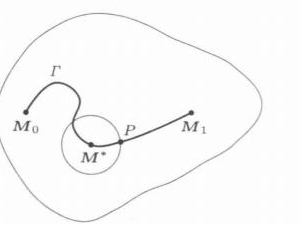
\includegraphics[width=.36\linewidth]{figures/lower/ch26/fig-26-1.png}

  图 26.1
\end{center}
但由平均值公式有
\[
  \frac{1}{4\pi\delta^2}\oiint_{\partial B_\delta(M^*)}u(x,y,z)\,\dd S=u(M^*)=K,
\]
由此得到矛盾。同理可证 $u$ 也不能在 $\Omega$ 的内点取得 $u$ 在 $\Omega$ 上的下界。
\end{xproof}

\begin{xremark}
1. 上述两个性质对任意维数的调和函数都是成立的。

2. 若 $\Omega$ 是有界区域，$u$ 在 $\overline\Omega$ 上连续，在 $\Omega$ 上调和，则 $u$ 的最大最小值只能在 $\Omega$ 的边界上达到。
\end{xremark}

\subsection{Poisson 积分公式}

在这一节我们证明，平面上每一个在单位圆周上的连续函数可惟一连续延拓成为单位开圆盘上的调和函数。为此设 $f(\theta)$ 是以 $2\pi$ 为周期的连续函数，我们要在单位圆盘上证明存在惟一的连续函数
\[
  u(r\cos\theta,r\sin\theta),
\]
当 $0\le r<1$ 时是调和函数，且
\[
  u(\cos\theta,\sin\theta)=f(\theta).
\]
证惟一性。设 $u,v$ 都满足条件，则 $w=u-v$ 当 $0\le r<1$ 时是调和函数，且
\[
  w(\cos\theta,\sin\theta)=0,\qquad 0\le\theta<2\pi.
\]
由极值原理（性质 2）知 $w\equiv0$，于是惟一性成立。

存在性的证明要困难得多。利用调和算子在极坐标系 $(r,\theta)$ 中的表达式
\[
  \Delta:=\frac{\partial^2}{\partial x^2}+\frac{\partial^2}{\partial y^2}
  =\frac{\partial^2}{\partial r^2}+\frac{1}{r}\frac{\partial}{\partial r}
  +\frac{1}{r^2}\frac{\partial^2}{\partial\theta^2},
\]
容易证明 $\Delta(r^n\cos n\theta)=\Delta(r^n\sin n\theta)=0$，$n=0,1,2,\ldots$。由此，我们令
\[
  u(r\cos\theta,r\sin\theta)
  =\frac{a_0}{2}+\sum_{n=1}^\infty(a_n\cos n\theta+b_n\sin n\theta)r^n.
\]
令 $r=1$，由已知条件得到
\[
  f(\theta)=\frac{a_0}{2}+\sum_{n=1}^\infty(a_n\cos n\theta+b_n\sin n\theta).
\]
由周期函数的 Fourier 级数理论知
\[
  a_n=\frac{1}{\pi}\int_0^{2\pi}f(\varphi)\cos n\varphi\,\dd\varphi,
  \qquad
  b_n=\frac{1}{\pi}\int_0^{2\pi}f(\varphi)\sin n\varphi\,\dd\varphi,
\]
代入 $u$ 的表达式中得到
\begin{align*}
  u(r\cos\theta,r\sin\theta)
  &=\frac{1}{\pi}\int_0^{2\pi}f(\varphi)
  \left[\frac12+\sum_{n=1}^\infty r^n\cos n(\theta-\varphi)\right]\,\dd\varphi\\
  &=\frac{1}{2\pi}\int_0^{2\pi}f(\varphi)\operatorname{Re}
  \left[\frac{1+r\ee^{\ii(\theta-\varphi)}}{1-r\ee^{\ii(\theta-\varphi)}}\right]\,\dd\varphi\\
  &=\frac{1}{2\pi}\int_0^{2\pi}f(\varphi)
  \frac{1-r^2}{1-2r\cos(\theta-\varphi)+r^2}\,\dd\varphi.
\end{align*}
下面证明它的确提供了问题的解。

首先证明 $u$ 在单位圆盘上是调和函数，这只是一个对含参变量常义积分求二阶偏导数的计算，所以留作练习，其中要将 $u$ 的表达式改写为
\[
  u(x,y)=\frac{1}{2\pi}\int_0^{2\pi}f(\varphi)
  \frac{1-x^2-y^2}{1-2(x\cos\varphi+y\sin\varphi)+x^2+y^2}\,\dd\varphi.
\]
最后证明对每一个 $\theta_0$，
\[
  \lim_{(\theta,r)\to(\theta_0,1^-)}\frac{1}{2\pi}\int_0^{2\pi}f(\varphi)
  \frac{1-r^2}{1-2r\cos(\theta-\varphi)+r^2}\,\dd\varphi=f(\theta_0),
\]
这件事我们已经在例题 18.2.4 中证明过了。这就完成了下面命题的证明。

\begin{xproposition}[26.2.1]
若 $f$ 是以 $2\pi$ 为周期的连续函数，则
\[
  u(r\cos\theta,r\sin\theta)
  =\frac{1}{2\pi}\int_0^{2\pi}f(\varphi)
  \frac{1-r^2}{1-2r\cos(\theta-\varphi)+r^2}\,\dd\varphi
\]
是单位圆盘上的调和函数，且
\[
  \lim_{(\theta,r)\to(\theta_0,1^-)}\frac{1}{2\pi}\int_0^{2\pi}f(\varphi)
  \frac{1-r^2}{1-2r\cos(\theta-\varphi)+r^2}\,\dd\varphi=f(\theta_0).
\]
\end{xproposition}

\paragraph{推论}
若 $u$ 是半径为 $R>0$ 的圆盘上的调和函数，则对于 $0\le r<R$ 有
\begin{equation}
  \begin{aligned}
  u(r\cos\theta,r\sin\theta)
  =\frac{1}{2\pi}\int_0^{2\pi}u(R\cos\varphi,R\sin\varphi)
  \frac{R^2-r^2}{R^2-2Rr\cos(\theta-\varphi)+r^2}\,\dd\varphi.
  \end{aligned}
  \tag{26.20}
  \label{eq:26.20}
\end{equation}
称 (26.20) 为 \textbf{Poisson 积分公式}。

\begin{xproof}
若 $R=1$，结论就是命题 26.2.1。对于一般情形只需作一相似变换，具体细节留作练习。
\end{xproof}

\subsection{练习题}

\begin{xexercise}[1]
证明：
\begin{enumerate}[label=(\arabic*)]
  \item $\nabla\times(\nabla f)=0$；
  \item $\nabla(\nabla\cdot\vect{a})-\nabla\times(\nabla\times\vect{a})=\Delta\vect{a}$，其中 $\Delta\vect{a}=(\Delta a_1,\Delta a_2,\Delta a_3)$。
\end{enumerate}
\end{xexercise}
\begin{xsolution}
\begin{enumerate}[label=(\arabic*)]
  \item 设 $f$ 二阶连续可微，则
  \[
    \nabla\times(\nabla f)
    =\left(
      f_{zy}-f_{yz},
      f_{xz}-f_{zx},
      f_{yx}-f_{xy}
    \right)=\vect{0}.
  \]

  \item 设 $\vect{a}=(a_1,a_2,a_3)$。考察第一分量：
  \begin{align*}
    [\nabla(\nabla\cdot\vect{a})]_1
    &=a_{1,xx}+a_{2,yx}+a_{3,zx},\\
    [\nabla\times(\nabla\times\vect{a})]_1
    &=\frac{\partial}{\partial y}(a_{2,x}-a_{1,y})
      -\frac{\partial}{\partial z}(a_{1,z}-a_{3,x})\\
    &=a_{2,xy}-a_{1,yy}-a_{1,zz}+a_{3,xz}.
  \end{align*}
  由混合偏导数相等，二者相减得到
  \[
    a_{1,xx}+a_{1,yy}+a_{1,zz}=\Delta a_1.
  \]
  对第二、第三分量作同样计算，便有
  \[
    \nabla(\nabla\cdot\vect{a})-\nabla\times(\nabla\times\vect{a})
    =(\Delta a_1,\Delta a_2,\Delta a_3)
    =\Delta\vect{a}.
  \]
\end{enumerate}
\end{xsolution}


\begin{xexercise}[2]
（\textbf{第二 Green 恒等式}）设 $\Sigma$ 为分片光滑封闭曲面，围成的区域为 $\Omega$，$u,v$ 在 $\overline\Omega$ 上二次连续可微。证明：
\[
  \iiint_\Omega(v\Delta u-u\Delta v)\,\dd x\,\dd y\,\dd z
  =\oiint_\Sigma\left(v\frac{\partial u}{\partial n}-u\frac{\partial v}{\partial n}\right)\,\dd S,
\]
其中 $\vect{n}$ 为 $\Sigma$ 的单位外法向量。
\end{xexercise}
\begin{xsolution}
对 $u,v$ 使用第一 Green 恒等式，
\[
  \iiint_\Omega v\Delta u\,\dd V
  +\iiint_\Omega\nabla u\cdot\nabla v\,\dd V
  =\oiint_\Sigma v\frac{\partial u}{\partial n}\,\dd S.
\]
交换 $u,v$，得到
\[
  \iiint_\Omega u\Delta v\,\dd V
  +\iiint_\Omega\nabla v\cdot\nabla u\,\dd V
  =\oiint_\Sigma u\frac{\partial v}{\partial n}\,\dd S.
\]
第一式减去第二式，中间的梯度内积项抵消，故
\[
  \boxed{
  \iiint_\Omega(v\Delta u-u\Delta v)\,\dd V
  =\oiint_\Sigma\left(
  v\frac{\partial u}{\partial n}
  -u\frac{\partial v}{\partial n}
  \right)\,\dd S
  }.
\]
这就是第二 Green 恒等式。
\end{xsolution}


\begin{xexercise}[3]
$\Sigma$ 为分片光滑封闭曲面，围成的区域为 $\Omega$，$u$ 在 $\overline\Omega$ 上二次连续可微，在 $\Omega$ 上调和。证明：
\[
  \iiint_\Omega\abs{\nabla u}^2\,\dd x\,\dd y\,\dd z
  =\oiint_\Sigma u\frac{\partial u}{\partial n}\,\dd S,
\]
并由此证明调和函数的惟一性，即调和函数在 $\Omega$ 内部的值由它在边界 $\Sigma$ 上的值惟一确定。
\end{xexercise}
\begin{xsolution}
在第一 Green 恒等式中令 $v=u$，得到
\[
  \iiint_\Omega u\Delta u\,\dd V
  +\iiint_\Omega\abs{\nabla u}^2\,\dd V
  =\oiint_\Sigma u\frac{\partial u}{\partial n}\,\dd S.
\]
因 $u$ 在 $\Omega$ 上调和，$\Delta u=0$，于是
\[
  \boxed{
  \iiint_\Omega\abs{\nabla u}^2\,\dd V
  =\oiint_\Sigma u\frac{\partial u}{\partial n}\,\dd S
  }.
\]

下面证明惟一性。设 $u_1,u_2$ 都在 $\Omega$ 内调和并在边界 $\Sigma$ 上取相同的值，令
\[
  w=u_1-u_2.
\]
则
\[
  \Delta w=0\quad\text{于 }\Omega,
  \qquad
  w=0\quad\text{于 }\Sigma.
\]
把上面的等式用于 $w$，有
\[
  \iiint_\Omega\abs{\nabla w}^2\,\dd V
  =\oiint_\Sigma w\frac{\partial w}{\partial n}\,\dd S=0.
\]
被积函数非负且连续，所以 $\nabla w=\vect{0}$ 于 $\Omega$。若 $\Omega$ 连通，则 $w$ 为常数；又 $w$ 在边界为零，故 $w\equiv0$。因此
\[
  u_1\equiv u_2,
\]
即调和函数在内部的值由边界值惟一确定。
\end{xsolution}


\begin{xexercise}[4]
在调和函数性质 1 的条件下，证明：
\[
  u(M_0)=\frac{1}{\frac43\pi R^3}\iiint_{B_R(M_0)}u(x,y,z)\,\dd x\,\dd y\,\dd z.
\]
\end{xexercise}
\begin{xsolution}
由调和函数的球面平均值公式，对每个 $0<\rho\le R$，
\[
  \oiint_{\partial B_\rho(M_0)}u\,\dd S
  =4\pi\rho^2u(M_0).
\]
按以 $M_0$ 为中心的球坐标逐层积分，
\begin{align*}
  \iiint_{B_R(M_0)}u(x,y,z)\,\dd V
  &=\int_0^R\left(
    \oiint_{\partial B_\rho(M_0)}u\,\dd S
    \right)\dd\rho\\
  &=4\pi u(M_0)\int_0^R\rho^2\,\dd\rho\\
  &=\frac{4}{3}\pi R^3u(M_0).
\end{align*}
所以
\[
  \boxed{
  u(M_0)=\frac{1}{\frac43\pi R^3}
  \iiint_{B_R(M_0)}u(x,y,z)\,\dd x\,\dd y\,\dd z
  }.
\]
\end{xsolution}


\begin{xexercise}[5]
证明命题 26.2.1 的推论。
\end{xexercise}
\begin{xsolution}
设 $u$ 在半径为 $R$ 的圆盘内调和。定义单位圆盘上的函数
\[
  v(\rho\cos\theta,\rho\sin\theta)
  =u(R\rho\cos\theta,R\rho\sin\theta),
  \qquad 0\le\rho<1.
\]
因为
\[
  \Delta v=R^2(\Delta u)\circ(R\,\cdot)=0,
\]
故 $v$ 在单位圆盘上调和。由命题 26.2.1，若 $s=r/R$，则
\begin{align*}
  u(r\cos\theta,r\sin\theta)
  &=v(s\cos\theta,s\sin\theta)\\
  &=\frac{1}{2\pi}\int_0^{2\pi}
    v(\cos\varphi,\sin\varphi)
    \frac{1-s^2}{1-2s\cos(\theta-\varphi)+s^2}\,\dd\varphi\\
  &=\frac{1}{2\pi}\int_0^{2\pi}
    u(R\cos\varphi,R\sin\varphi)
    \frac{R^2-r^2}{R^2-2Rr\cos(\theta-\varphi)+r^2}\,\dd\varphi.
\end{align*}
这正是 Poisson 积分公式 (26.20)。
\end{xsolution}


\begin{xexercise}[6]
证明：Poisson 积分公式 (26.20) 定义的函数是调和函数。
\end{xexercise}
\begin{xsolution}
记
\[
  q=\frac{r}{R},\qquad 0\le q<1.
\]
Poisson 核可展开为
\begin{align*}
  \frac{R^2-r^2}{R^2-2Rr\cos(\theta-\varphi)+r^2}
  &=\frac{1-q^2}{1-2q\cos(\theta-\varphi)+q^2}\\
  &=1+2\sum_{n=1}^\infty q^n\cos n(\theta-\varphi).
\end{align*}
对任意固定的 $0<\rho<R$，当 $r\le\rho$ 时，不但上式级数一致收敛，而且把它对 $x,y$ 求至二阶偏导所得级数也一致收敛，因为相应项可由常数倍的
\[
  n^2\left(\frac{\rho}{R}\right)^{n-2}
\]
控制，而该数项级数收敛。因此可以在积分号与级数号下逐项求二阶偏导。

对固定的 $\varphi$，每一项
\[
  r^n\cos n(\theta-\varphi)
\]
都是 $x,y$ 的调和多项式的线性组合，故其 Laplace 算子为零，常数项也显然调和。于是 Poisson 公式定义的函数满足
\[
  \Delta u(x,y)
  =\frac{1}{2\pi}\int_0^{2\pi}
  f(\varphi)\,\Delta_{x,y}
  \left[
  \frac{R^2-r^2}{R^2-2Rr\cos(\theta-\varphi)+r^2}
  \right]\dd\varphi=0
\]
于任意闭圆盘 $r\le\rho<R$。由于 $\rho$ 任意，$u$ 在整个开圆盘 $r<R$ 上调和。
\end{xsolution}


\begin{xexercise}[7]
证明：调和函数无限次可微。
\end{xexercise}
\begin{xsolution}
给出一个同时适用于二维和三维的证明。设 $u$ 在区域 $\Omega$ 上调和，取任意 $x_0\in\Omega$，再取 $\varepsilon>0$ 使
\[
  \overline{B_{2\varepsilon}(x_0)}\subset\Omega.
\]
取一个非负、径向对称的 $C^\infty$ 函数 $\eta_\varepsilon$，其支集包含于 $B_\varepsilon(0)$ 且
\[
  \int\eta_\varepsilon(y)\,\dd y=1.
\]
对 $x\in B_\varepsilon(x_0)$，由调和函数的球面平均值公式，把积分按半径分层可得
\begin{align*}
  (u*\eta_\varepsilon)(x)
  &=\int_{B_\varepsilon(0)}u(x-y)\eta_\varepsilon(y)\,\dd y\\
  &=u(x)\int_{B_\varepsilon(0)}\eta_\varepsilon(y)\,\dd y
  =u(x).
\end{align*}
这里第二个等号的理由是：在每个固定半径的球面上，$u(x-y)$ 的平均值都等于 $u(x)$，而 $\eta_\varepsilon$ 在该球面上为常数。

卷积 $u*\eta_\varepsilon$ 是 $C^\infty$ 函数，因此 $u$ 在 $B_\varepsilon(x_0)$ 上无限次可微。由于 $x_0$ 任意，$u\in C^\infty(\Omega)$。
\end{xsolution}


\begin{xexercise}[8]
若 $f$ 和 $g\circ f$ 都是一连通开集上的调和函数，$g$ 二阶连续可微，$f$ 不是常值函数，证明：$g$ 是线性函数。
\end{xexercise}
\begin{xsolution}
设定义域为连通开集 $G$。由 $f$ 与 $g\circ f$ 都调和，
\[
  \Delta f=0,
  \qquad
  \Delta(g(f))=0.
\]
利用复合函数求导公式，
\begin{align*}
  \Delta(g(f))
  &=g''(f)\abs{\nabla f}^2+g'(f)\Delta f\\
  &=g''(f)\abs{\nabla f}^2.
\end{align*}
故
\begin{equation}
  g''(f(x))\abs{\nabla f(x)}^2=0,
  \qquad x\in G.
  \tag{*}
\end{equation}

下面证明 $g''$ 在 $f(G)$ 上恒为零。反设存在 $x_0\in G$ 使
\[
  g''(f(x_0))\ne0.
\]
由 $g''$ 连续，可取含 $f(x_0)$ 的开区间 $I$，使 $g''$ 在 $I$ 上处处不为零。令 $U$ 为开集
\[
  \{x\in G\mid f(x)\in I\}
\]
中含 $x_0$ 的连通分支。由 (*)，在 $U$ 上必有 $\nabla f=0$，所以 $f$ 在 $U$ 上为常数，且等于 $f(x_0)$。

若 $U$ 在 $G$ 中有边界点 $p$，由连续性 $f(p)=f(x_0)\in I$。于是 $p$ 的某个小邻域仍包含于 $f^{-1}(I)$，且与 $U$ 相交，这与 $U$ 是 $f^{-1}(I)$ 的连通分支矛盾。因此 $U$ 在 $G$ 中既开又闭。由于 $G$ 连通，只能有 $U=G$，从而 $f$ 为常值函数，与题设矛盾。

因此 $g''(t)=0$ 对每个 $t\in f(G)$ 都成立。又因为连通集 $G$ 的连续像 $f(G)$ 是区间，所以在该区间上
\[
  g(t)=at+b.
\]
即 $g$ 在 $f(G)$ 上是线性函数（仿射函数）。
\end{xsolution}


\begin{xexercise}[9]
证明：问题
\[
  \Delta u=f(x,y,z),\quad (x,y,z)\in D,
  \qquad
  \frac{\partial u}{\partial n}=g(x,y,z),\quad (x,y,z)\in\partial D
\]
有解 $u$ 的必要条件是
\[
  \iiint_D f\,\dd x\,\dd y\,\dd z=\oiint_{\partial D}g\,\dd S.
\]
\end{xexercise}
\begin{xsolution}
若问题有解 $u$，则由 Gauss 公式，
\begin{align*}
  \iiint_D f\,\dd x\,\dd y\,\dd z
  &=\iiint_D\Delta u\,\dd x\,\dd y\,\dd z\\
  &=\oiint_{\partial D}\nabla u\cdot\vect{n}\,\dd S\\
  &=\oiint_{\partial D}\frac{\partial u}{\partial n}\,\dd S\\
  &=\oiint_{\partial D}g\,\dd S.
\end{align*}
所以
\[
  \boxed{
  \iiint_D f\,\dd x\,\dd y\,\dd z
  =\oiint_{\partial D}g\,\dd S
  }
\]
是该 Neumann 问题有解的必要条件。
\end{xsolution}


\section{对于教学的建议}

\subsection{学习要点}

\begin{enumerate}[label=\arabic*.]
  \item 本章涉及的定义和概念较多。定义了散度、旋度之后，Green 公式、Gauss 公式与 Stokes 公式从表面上看是简单化了。散度定理 (26.5)（或者是 (26.2)，(26.4)）的用处非常之广，当需要证明重积分与曲线（面）积分具有某种关系时，散度定理是一个非常有效的出发点。
  \item 由于 Laplace 算子对一个函数的作用等于这个函数的梯度的散度，因此当积分号后面出现 Laplace 算子，再应用散度定理时，各类积分变得丰富多彩，能够熟练运用 Laplace 算符与散度定理是本章的主要目的之一。
  \item 调和函数是一类性质非常好的函数，调和二字表现在处处满足平均值公式，事实上反过来的结论也成立，即处处满足平均值公式的连续函数一定是调和函数（见第二组参考题 1）。在本章只介绍了调和函数的一点基本知识，在复变函数、数学物理方程等后续课程中还要进一步学习。
  \item \textbf{对于习题课教学的建议}
  \begin{enumerate}[label=(\arabic*)]
    \item 在习题课上证明命题 26.1.1，虽然题目并不难，但却是对各种算子的定义、各种场的定义、Green 公式、Gauss 公式、Stokes 公式、曲线积分与路径无关的一个综合练习。
    \item 关于 Laplace 算子，要求学生会证明第一和第二 Green 恒等式。
    \item 关于调和函数，要求学生会证明平均值公式，并能利用 Poisson 积分公式证明调和函数的一些性质。
  \end{enumerate}
\end{enumerate}

\subsection{参考题}

\paragraph{第一组参考题}

\begin{xreferenceproblem}[1]
设 $\vect{A},\vect{B}$ 为光滑向量场。证明：
\begin{enumerate}[label=(\arabic*)]
  \item $\nabla(\vect{A}\cdot\vect{B})=\vect{A}\times(\nabla\times\vect{B})+\vect{B}\times(\nabla\times\vect{A})+(\vect{B}\cdot\nabla)\vect{A}+(\vect{A}\cdot\nabla)\vect{B}$；
  \item $\nabla\times(\vect{A}\times\vect{B})=(\vect{B}\cdot\nabla)\vect{A}-(\vect{A}\cdot\nabla)\vect{B}+(\nabla\cdot\vect{B})\vect{A}-(\nabla\cdot\vect{A})\vect{B}$。
\end{enumerate}
\end{xreferenceproblem}
\begin{xsolution}
记 $\varepsilon_{ijk}$ 为 Levi--Civita 符号，$\delta_{ij}$ 为 Kronecker 符号，并采用重复指标求和约定。用恒等式
\[
  \varepsilon_{ijk}\varepsilon_{klm}
  =\delta_{il}\delta_{jm}-\delta_{im}\delta_{jl}.
\]

\begin{enumerate}[label=(\arabic*)]
  \item 第 $i$ 个分量有
  \begin{align*}
    [\vect{A}\times(\nabla\times\vect{B})]_i
    &=\varepsilon_{ijk}A_j\varepsilon_{klm}\partial_lB_m\\
    &=A_m\partial_iB_m-A_l\partial_lB_i,
  \end{align*}
  同理
  \[
    [\vect{B}\times(\nabla\times\vect{A})]_i
    =B_m\partial_iA_m-B_l\partial_lA_i.
  \]
  再加上
  \[
    [(\vect{B}\cdot\nabla)\vect{A}]_i=B_l\partial_lA_i,
    \qquad
    [(\vect{A}\cdot\nabla)\vect{B}]_i=A_l\partial_lB_i,
  \]
  后两组项恰好抵消，留下
  \[
    A_m\partial_iB_m+B_m\partial_iA_m
    =\partial_i(\vect{A}\cdot\vect{B}).
  \]
  三个分量都成立，故
  \[
    \nabla(\vect{A}\cdot\vect{B})
    =\vect{A}\times(\nabla\times\vect{B})
    +\vect{B}\times(\nabla\times\vect{A})
    +(\vect{B}\cdot\nabla)\vect{A}
    +(\vect{A}\cdot\nabla)\vect{B}.
  \]

  \item 第 $i$ 个分量为
  \begin{align*}
    [\nabla\times(\vect{A}\times\vect{B})]_i
    &=\varepsilon_{ijk}\partial_j(\varepsilon_{klm}A_lB_m)\\
    &=\partial_m(A_iB_m)-\partial_l(A_lB_i)\\
    &=B_m\partial_mA_i-A_l\partial_lB_i
      +(\partial_mB_m)A_i-(\partial_lA_l)B_i.
  \end{align*}
  因此
  \[
    \nabla\times(\vect{A}\times\vect{B})
    =(\vect{B}\cdot\nabla)\vect{A}
    -(\vect{A}\cdot\nabla)\vect{B}
    +(\nabla\cdot\vect{B})\vect{A}
    -(\nabla\cdot\vect{A})\vect{B}.
  \]
\end{enumerate}
\end{xsolution}


\begin{xreferenceproblem}[2]
设 $G$ 是 $\RR^3$ 中关于原点 $O$ 的星形区域，$\vect{F}(x,y,z)$ 为 $G$ 上的光滑无旋场。定义
\[
  \vect{A}(x,y,z)=\int_0^1\bigl[t\vect{F}(tx,ty,tz)\times\vect{r}\bigr]\,\dd t.
\]
利用上题 (2) 证明：
\[
  \nabla\times\vect{A}=\vect{F}.
\]
\end{xreferenceproblem}
\begin{xsolution}
按原书题意，$\vect{F}$ 是无源场，即
\[
  \nabla\cdot\vect{F}=0.
\]
令 $\vect{r}=(x,y,z)$。对固定的 $t\in[0,1]$，在上一题 (2) 中取
\[
  \vect{X}(\vect{r})=t\vect{F}(t\vect{r}),
  \qquad
  \vect{Y}(\vect{r})=\vect{r}.
\]
因为
\[
  (\vect{X}\cdot\nabla)\vect{r}=\vect{X},
  \qquad
  \nabla\cdot\vect{r}=3,
\]
且
\[
  \nabla\cdot\vect{X}
  =t^2(\nabla\cdot\vect{F})(t\vect{r})=0,
\]
故上一题 (2) 给出
\begin{align*}
  \nabla\times[t\vect{F}(t\vect{r})\times\vect{r}]
  &=(\vect{r}\cdot\nabla)[t\vect{F}(t\vect{r})]
    -t\vect{F}(t\vect{r})+3t\vect{F}(t\vect{r})\\
  &=t^2(\vect{r}\cdot\nabla)\vect{F}(t\vect{r})
    +2t\vect{F}(t\vect{r})\\
  &=\frac{\dd}{\dd t}\left[t^2\vect{F}(t\vect{r})\right].
\end{align*}
于是可以在积分号下取旋度：
\begin{align*}
  \nabla\times\vect{A}(\vect{r})
  &=\int_0^1
    \nabla\times[t\vect{F}(t\vect{r})\times\vect{r}]\,\dd t\\
  &=\int_0^1\frac{\dd}{\dd t}
    [t^2\vect{F}(t\vect{r})]\,\dd t\\
  &=\vect{F}(\vect{r})-\lim_{t\to0^+}t^2\vect{F}(t\vect{r})\\
  &=\vect{F}(\vect{r}),
\end{align*}
因为 $\vect{F}$ 在原点附近光滑有界。因此
\[
  \boxed{\nabla\times\vect{A}=\vect{F}}.
\]
\end{xsolution}


\begin{xreferenceproblem}[3]
设 $\vect{A}$ 是 $\RR^3$ 上的光滑向量场，$\vect{B}$ 是 $\RR^3$ 上二次连续可微的向量场，满足
\[
  \nabla\times\vect{B}=\frac{1}{r}(\nabla r\times\vect{A}),
\]
其中 $r=\sqrt{x^2+y^2+z^2}$，证明：
\[
  \oint_L\vect{A}\cdot\vect{\tau}\,\dd s=0,
\]
其中 $L$ 是以原点为中心的球面上的封闭光滑简单定向曲线，$\vect{\tau}$ 是 $L$ 上与其方向一致的单位切向量。
\end{xreferenceproblem}
\begin{xsolution}
题设给出
\[
  \nabla\times\vect{B}=\frac1r(\nabla r\times\vect{A}),
  \qquad r=\sqrt{x^2+y^2+z^2}.
\]
对两边取散度。由旋度的散度为零，
\[
  0=\nabla\cdot\left[\frac1r(\nabla r\times\vect{A})\right].
\]
利用乘积公式，
\begin{align*}
  0
  &=\nabla\left(\frac1r\right)\cdot(\nabla r\times\vect{A})
    +\frac1r\nabla\cdot(\nabla r\times\vect{A}).
\end{align*}
其中 $\nabla(1/r)$ 与 $\nabla r$ 平行，故第一项为零；又由
\[
  \nabla\cdot(\vect{P}\times\vect{Q})
  =\vect{Q}\cdot(\nabla\times\vect{P})
  -\vect{P}\cdot(\nabla\times\vect{Q}),
\]
取 $\vect{P}=\nabla r$、$\vect{Q}=\vect{A}$，并用
\[
  \nabla\times(\nabla r)=\vect{0},
\]
得到
\[
  \nabla\cdot(\nabla r\times\vect{A})
  =-\nabla r\cdot(\nabla\times\vect{A}).
\]
因此
\[
  \nabla r\cdot(\nabla\times\vect{A})=0.
\]

设 $L$ 位于半径为 $R$ 的球面上，取该球面上由 $L$ 围成的一片定向曲面 $S$。在 $S$ 上单位法向量可取
\[
  \vect{n}=\nabla r.
\]
于是由 Stokes 公式，
\[
  \oint_L\vect{A}\cdot\vect{\tau}\,\dd s
  =\iint_S(\nabla\times\vect{A})\cdot\vect{n}\,\dd S
  =0.
\]
故
\[
  \boxed{\oint_L\vect{A}\cdot\vect{\tau}\,\dd s=0}.
\]
\end{xsolution}


\begin{xreferenceproblem}[4]
设长度为 $l$ 的平面简单闭曲线 $C$ 由方程 $F(x,y)=0$ 确定。$F(x,y)$ 二阶连续可微，且 $\nabla F(x,y)\ne0$，设
\[
  D=\{(x,y)\mid F(x,y)>0\}
\]
为曲线 $C$ 围成的区域，计算二重积分
\[
  \iint_D\nabla\cdot\left(\frac{\nabla F}{\abs{\nabla F}}\right)\,\dd x\,\dd y.
\]
\end{xreferenceproblem}
\begin{xsolution}
令
\[
  \vect{N}=\frac{\nabla F}{\abs{\nabla F}}.
\]
由二维散度定理（Green 公式），
\[
  \iint_D\nabla\cdot\vect{N}\,\dd x\,\dd y
  =\oint_C\vect{N}\cdot\vect{n}\,\dd s,
\]
其中 $\vect{n}$ 是 $D$ 的单位外法向量。

因为 $D=\{F>0\}$，在边界 $C$ 上，$\nabla F$ 指向 $F$ 增大的方向，即指向 $D$ 的内部。因此
\[
  \vect{n}=-\frac{\nabla F}{\abs{\nabla F}}=-\vect{N}.
\]
故
\[
  \vect{N}\cdot\vect{n}=-1.
\]
于是
\[
  \boxed{
  \iint_D\nabla\cdot\left(\frac{\nabla F}{\abs{\nabla F}}\right)\,\dd x\,\dd y
  =-\oint_C\dd s=-l
  }.
\]
\end{xsolution}


\begin{xreferenceproblem}[5]
设 $u(x,y,z)$ 是连续函数，它在 $M(x_0,y_0,z_0)$ 处有连续二阶偏导数，记
\[
  F(R)=\frac{1}{4\pi R^2}\oiint_{\partial B_R(M)}u(x,y,z)\,\dd S,
\]
其中 $\partial B_R(M)$ 是以 $M$ 为心、$R$ 为半径的球面。证明：
\[
  \lim_{R\to0}F(R)=u(M).
\]
若 $\Delta u(M)$ 不等于零，求无穷小量 $F(R)-u(M)$ 的主要部分。
\end{xreferenceproblem}
\begin{xsolution}
记 $M=(x_0,y_0,z_0)$，令 $\vect{\omega}$ 为单位球面上的单位向量。由球面面积的缩放关系，
\[
  F(R)=\frac{1}{4\pi}\oiint_{\partial B_1(0)}u(M+R\vect{\omega})\,\dd S_1.
\]
由 $u$ 在 $M$ 连续，$u(M+R\vect{\omega})\to u(M)$ 对 $\vect{\omega}$ 一致成立，因此
\[
  \lim_{R\to0^+}F(R)=u(M).
\]

下面求主要部分。由于 $u$ 在 $M$ 有连续二阶偏导数，Taylor 展开为
\[
  u(M+R\vect{\omega})
  =u(M)+R\nabla u(M)\cdot\vect{\omega}
  +\frac{R^2}{2}\vect{\omega}^{\mathsf T}H_u(M)\vect{\omega}
  +\littleo(R^2),
\]
其中余项对单位球面上的 $\vect{\omega}$ 一致。球面对称性给出
\[
  \frac1{4\pi}\oiint_{\partial B_1}\omega_i\,\dd S=0,
  \qquad
  \frac1{4\pi}\oiint_{\partial B_1}\omega_i\omega_j\,\dd S
  =\begin{cases}
  \frac13,&i=j,\\
  0,&i\ne j.
  \end{cases}
\]
因此
\begin{align*}
  F(R)-u(M)
  &=\frac{R^2}{2}\cdot\frac13
  \left(u_{xx}(M)+u_{yy}(M)+u_{zz}(M)\right)
  +\littleo(R^2)\\
  &=\frac{\Delta u(M)}{6}R^2+\littleo(R^2).
\end{align*}
若 $\Delta u(M)\ne0$，则无穷小量 $F(R)-u(M)$ 的主要部分为
\[
  \boxed{\frac{\Delta u(M)}6R^2}.
\]
\end{xsolution}


\begin{xreferenceproblem}[6]
设 $u,v$ 在 $\overline\Omega$ 上二阶连续可微，且在 $\Omega$ 的边界上 $u=v$。如果 $u$ 是调和函数，则
\[
  \iiint_\Omega\abs{\nabla u}^2\,\dd x\,\dd y\,\dd z
  \le\iiint_\Omega\abs{\nabla v}^2\,\dd x\,\dd y\,\dd z.
\]
\end{xreferenceproblem}
\begin{xsolution}
令
\[
  w=v-u.
\]
由于 $u=v$ 于 $\partial\Omega$，有 $w=0$ 于 $\partial\Omega$。展开
\begin{align*}
  \iiint_\Omega\abs{\nabla v}^2\,\dd V
  &=\iiint_\Omega\abs{\nabla u+\nabla w}^2\,\dd V\\
  &=\iiint_\Omega\abs{\nabla u}^2\,\dd V
    +2\iiint_\Omega\nabla u\cdot\nabla w\,\dd V
    +\iiint_\Omega\abs{\nabla w}^2\,\dd V.
\end{align*}
由第一 Green 恒等式，
\[
  \iiint_\Omega\nabla u\cdot\nabla w\,\dd V
  =\oiint_{\partial\Omega}w\frac{\partial u}{\partial n}\,\dd S
  -\iiint_\Omega w\Delta u\,\dd V=0,
\]
因为 $w=0$ 于边界且 $u$ 调和。故
\[
  \iiint_\Omega\abs{\nabla v}^2\,\dd V
  =\iiint_\Omega\abs{\nabla u}^2\,\dd V
  +\iiint_\Omega\abs{\nabla w}^2\,\dd V
  \ge\iiint_\Omega\abs{\nabla u}^2\,\dd V.
\]
即得所证不等式。
\end{xsolution}


\begin{xreferenceproblem}[7]
设 $u(x,y)$ 在 $x^2+y^2<1$ 二阶连续可微，且 $\Delta u=\ee^{-(x^2+y^2)}$，证明：
\[
  \iint_{x^2+y^2<1}\left(x\frac{\partial u}{\partial x}+y\frac{\partial u}{\partial y}\right)\,\dd x\,\dd y
  =\frac{\pi}{2\ee}.
\]
\end{xreferenceproblem}
\begin{xsolution}
令
\[
  x=r\cos\theta,
  \qquad
  y=r\sin\theta,
  \qquad
  0\le r<1.
\]
则
\[
  x\frac{\partial u}{\partial x}
  +y\frac{\partial u}{\partial y}
  =r\frac{\partial u}{\partial r}.
\]
因此所求积分为
\begin{equation}
  I=\int_0^1\int_0^{2\pi}r^2u_r(r,\theta)\,\dd\theta\,\dd r.
  \tag{1}
\end{equation}

固定 $0<r<1$，在圆盘 $B_r=\{x^2+y^2<r^2\}$ 上应用 Green 公式：
\begin{align*}
  \oint_{\partial B_r}
  \left(u_x\,\dd y-u_y\,\dd x\right)
  &=\iint_{B_r}\Delta u\,\dd x\,\dd y\\
  &=\iint_{B_r}\ee^{-(x^2+y^2)}\,\dd x\,\dd y\\
  &=2\pi\int_0^r\rho\ee^{-\rho^2}\,\dd\rho\\
  &=\pi(1-\ee^{-r^2}).
\end{align*}
在圆周 $\partial B_r$ 上有
\[
  \dd x=-r\sin\theta\,\dd\theta,
  \qquad
  \dd y=r\cos\theta\,\dd\theta,
\]
故左端等于
\[
  \int_0^{2\pi}r
  \left(u_x\cos\theta+u_y\sin\theta\right)\,\dd\theta
  =\int_0^{2\pi}r u_r(r,\theta)\,\dd\theta.
\]
于是
\[
  \int_0^{2\pi}r u_r(r,\theta)\,\dd\theta
  =\pi(1-\ee^{-r^2}).
\]
代入 (1)，得到
\begin{align*}
  I
  &=\pi\int_0^1 r(1-\ee^{-r^2})\,\dd r\\
  &=\frac{\pi}{2}-\frac{\pi}{2}(1-\ee^{-1})\\
  &=\frac{\pi}{2\ee}.
\end{align*}
故
\[
  \boxed{I=\frac{\pi}{2\ee}}.
\]
\end{xsolution}


\paragraph{第二组参考题}

\begin{xreferenceproblem}[1]
证明：处处满足平均值公式的连续函数一定是调和函数。
\end{xreferenceproblem}
\begin{xsolution}
取任意闭球
\[
  \overline{G}\subset\Omega.
\]
以 $u$ 在 $\partial G$ 上的值为边值，用球上的 Poisson 积分公式定义函数 $v$。则 $v$ 在 $G$ 内调和，在 $\overline G$ 上连续，并且
\[
  v=u\qquad\text{于 }\partial G.
\]
调和函数满足平均值公式，所以 $v$ 满足平均值公式；题设又说明 $u$ 满足平均值公式。因此
\[
  w=u-v
\]
也满足平均值公式，且
\[
  w=0\qquad\text{于 }\partial G.
\]

先说明满足平均值公式的连续函数同样满足极值原理。若 $w$ 在 $G$ 内某点 $P$ 取得正的最大值 $M$，则对任意充分小的 $r>0$，
\[
  M=w(P)=\frac{1}{\abs{\partial B_r(P)}}
  \int_{\partial B_r(P)}w\,\dd S.
\]
由于球面上处处有 $w\le M$，上式只能在整个球面上 $w=M$ 时成立。让 $r$ 在允许范围内变化，可知 $P$ 的一个邻域上均有 $w=M$。因此最大值点集既开又闭；由 $G$ 连通且边界上 $w=0$，不可能有 $M>0$。同理，$w$ 也不可能在内部取得负的最小值。于是
\[
  w\equiv0\qquad\text{于 }G.
\]
故 $u=v$ 于 $G$，从而 $u$ 在 $G$ 内调和。

由于 $G$ 可任取，得到
\[
  \Delta u=0\qquad\text{于 }\Omega,
\]
即 $u$ 是调和函数。
\end{xsolution}


\begin{xreferenceproblem}[2]
设 $u_n(x,y)$ 是定义在圆盘 $B_R$ 上的调和函数序列，都在 $\overline{B_R}$ 上连续，若 $u_n(x,y)$ 在 $B_R$ 的边界 $\partial B_R$ 上一致收敛，则 $u_n(x,y)$ 在 $\overline{B_R}$ 上也一致收敛，并且极限函数也是调和函数。
\end{xreferenceproblem}
\begin{xsolution}
由边界上的一致收敛，$u_n$ 在 $\partial B_R$ 上一致 Cauchy。对任意 $m,n$，函数
\[
  w_{m,n}=u_m-u_n
\]
在 $B_R$ 上调和并在闭圆盘上连续。由调和函数的极值原理分别用于 $w_{m,n}$ 与 $-w_{m,n}$，
\[
  \sup_{\overline{B_R}}\abs{u_m-u_n}
  \le\sup_{\partial B_R}\abs{u_m-u_n}.
\]
右端随 $m,n\to\infty$ 趋于零，所以 $u_n$ 在 $\overline{B_R}$ 上一致 Cauchy，从而一致收敛到某个连续函数 $u$。

还需证明 $u$ 调和。任取闭圆盘
\[
  \overline{B_\rho(P)}\subset B_R.
\]
每个 $u_n$ 都满足平均值公式
\[
  u_n(P)=\frac{1}{2\pi}\int_0^{2\pi}u_n(P+\rho\vect{e}_\theta)\,\dd\theta.
\]
由一致收敛可以令 $n\to\infty$ 穿过积分号，得到
\[
  u(P)=\frac{1}{2\pi}\int_0^{2\pi}u(P+\rho\vect{e}_\theta)\,\dd\theta.
\]
因此 $u$ 处处满足平均值公式。由第二组参考题 1，$u$ 是调和函数。
\end{xsolution}


\begin{xreferenceproblem}[3]
设 $u(x,y,z)$ 在区域 $D$ 上二阶连续可微，证明：$\Delta u\ge0$（$\forall(x,y,z)\in D$）的充分必要条件是
\[
  u(M_0)\le\frac{1}{4\pi R^2}\oiint_{\partial B_R(M_0)}u(x,y,z)\,\dd S,
  \qquad \forall B_R(M_0)\subset D.
\]
\end{xreferenceproblem}
\begin{xsolution}
固定任意 $M_0\in D$，并定义球面平均值
\[
  F(R)=\frac{1}{4\pi R^2}\oiint_{\partial B_R(M_0)}u\,\dd S,
\]
其中 $B_R(M_0)\subset D$。与例题 26.2.2 的 (26.18) 同样计算可得
\begin{equation}
  F'(R)=\frac{1}{4\pi R^2}\iiint_{B_R(M_0)}\Delta u\,\dd V.
  \tag{1}
\end{equation}
并且由连续性
\[
  \lim_{R\to0^+}F(R)=u(M_0).
\]

若 $\Delta u\ge0$ 于 $D$，则由 (1) 有 $F'(R)\ge0$，所以
\[
  F(R)\ge F(0)=u(M_0),
\]
即
\[
  u(M_0)\le\frac{1}{4\pi R^2}
  \oiint_{\partial B_R(M_0)}u\,\dd S.
\]

反过来，假设上述不等式对所有闭球都成立。若存在一点 $M_0$ 使
\[
  \Delta u(M_0)<0,
\]
由连续性可取 $R_0>0$，使 $B_{R_0}(M_0)\subset D$ 且球内 $\Delta u<0$。于是对 $0<R<R_0$，由 (1)
\[
  F'(R)<0.
\]
故 $F(R)<F(0)=u(M_0)$，与题设平均值不等式矛盾。因此不存在这样的点，必有
\[
  \Delta u\ge0\quad\text{于 }D.
\]
充分性与必要性均得证。
\end{xsolution}


\begin{xreferenceproblem}[4]
设 $u(x,y,z)$ 是由光滑曲面 $S$ 所包围的有界区域 $\Omega$ 上的调和函数，则
\[
  u(x,y,z)=\frac{1}{4\pi}\oiint_S\left[
  u(\xi,\eta,\zeta)\frac{\cos(\vect{r},\vect{n})}{r^2}
  +\frac{1}{r}\frac{\partial u(\xi,\eta,\zeta)}{\partial n}
  \right]\,\dd S,
\]
其中 $\vect{r}=(\xi-x,\eta-y,\zeta-z)$，$r=\abs{\vect{r}}$。
\end{xreferenceproblem}
\begin{xsolution}
固定 $M=(x,y,z)\in\Omega$，积分变量记为
\[
  M'=(\xi,\eta,\zeta),
  \qquad
  \vect{r}=M'-M,
  \qquad
  r=\abs{\vect{r}}.
\]
函数 $1/r$ 在 $M'\ne M$ 时调和。取足够小的 $\varepsilon>0$，使闭球 $\overline{B_\varepsilon(M)}\subset\Omega$，并在穿孔区域
\[
  \Omega_\varepsilon=\Omega\setminus\overline{B_\varepsilon(M)}
\]
上对 $u$ 与 $1/r$ 使用第二 Green 恒等式。由于两者在 $\Omega_\varepsilon$ 上都调和，
\[
  0=\oiint_{\partial\Omega_\varepsilon}\left[
  \frac1r\frac{\partial u}{\partial n}
  -u\frac{\partial}{\partial n}\left(\frac1r\right)
  \right]\dd S.
\]
边界由外边界 $S$ 和内球面 $S_\varepsilon=\partial B_\varepsilon(M)$ 组成。

在外边界 $S$ 上，
\[
  \frac{\partial}{\partial n}\left(\frac1r\right)
  =\nabla_{M'}\left(\frac1r\right)\cdot\vect{n}
  =-\frac{\vect{r}\cdot\vect{n}}{r^3}
  =-\frac{\cos(\vect{r},\vect{n})}{r^2}.
\]
因此外边界贡献为
\[
  \oiint_S\left[
  \frac1r\frac{\partial u}{\partial n}
  +u\frac{\cos(\vect{r},\vect{n})}{r^2}
  \right]\dd S.
\]

注意在内球面上，作为穿孔区域 $\Omega_\varepsilon$ 的外法向量是径向向内的 $-\vect{e}_r$，故
\[
  \frac{\partial}{\partial n}\left(\frac1r\right)=\frac1{\varepsilon^2}.
\]
于是内球面贡献为
\[
  \oiint_{S_\varepsilon}\left[
  \frac1\varepsilon\frac{\partial u}{\partial n}
  -\frac{u}{\varepsilon^2}
  \right]\dd S.
\]
第一项的绝对值为 $\bigO(\varepsilon)$；第二项由 $u$ 的连续性满足
\[
  -\frac1{\varepsilon^2}\oiint_{S_\varepsilon}u\,\dd S
  \longrightarrow-4\pi u(M).
\]
令 $\varepsilon\to0^+$，得到
\[
  \oiint_S\left[
  \frac1r\frac{\partial u}{\partial n}
  +u\frac{\cos(\vect{r},\vect{n})}{r^2}
  \right]\dd S
  =4\pi u(M).
\]
故
\[
  \boxed{
  u(x,y,z)=\frac1{4\pi}\oiint_S\left[
  u(\xi,\eta,\zeta)\frac{\cos(\vect{r},\vect{n})}{r^2}
  +\frac1r\frac{\partial u(\xi,\eta,\zeta)}{\partial n}
  \right]\dd S
  }.
\]
\end{xsolution}


\begin{xreferenceproblem}[5]
利用 Poisson 积分公式证明不等式
\[
  \frac{R-r}{R+r}u(x_0,y_0)\le u(x,y)\le\frac{R+r}{R-r}u(x_0,y_0),
\]
其中 $u$ 是以 $R$ 为半径、$(x_0,y_0)$ 为圆心的开圆盘上的非负调和函数，$r<R$ 是 $(x,y)$ 与 $(x_0,y_0)$ 的距离。
\end{xreferenceproblem}
\begin{xsolution}
先把圆心平移到原点。设 $u$ 在 $B_R(0)$ 上非负调和，点 $(x,y)$ 的极坐标为 $(r,\theta)$。若 $u$ 未必连续到半径 $R$ 的边界，则先固定任意
\[
  r<\rho<R.
\]
在闭圆盘 $\overline{B_\rho(0)}$ 上应用 Poisson 公式：
\[
  u(r,\theta)=\frac1{2\pi}\int_0^{2\pi}
  u(\rho,\varphi)
  \frac{\rho^2-r^2}{\rho^2-2\rho r\cos(\theta-\varphi)+r^2}\,\dd\varphi.
\]
由于
\[
  (\rho-r)^2
  \le \rho^2-2\rho r\cos(\theta-\varphi)+r^2
  \le(\rho+r)^2,
\]
Poisson 核满足
\[
  \frac{\rho-r}{\rho+r}
  \le
  \frac{\rho^2-r^2}{\rho^2-2\rho r\cos(\theta-\varphi)+r^2}
  \le
  \frac{\rho+r}{\rho-r}.
\]
又 $u(\rho,\varphi)\ge0$，所以积分后
\[
  \frac{\rho-r}{\rho+r}\cdot
  \frac1{2\pi}\int_0^{2\pi}u(\rho,\varphi)\,\dd\varphi
  \le u(r,\theta)
  \le
  \frac{\rho+r}{\rho-r}\cdot
  \frac1{2\pi}\int_0^{2\pi}u(\rho,\varphi)\,\dd\varphi.
\]
由中心的平均值公式，
\[
  \frac1{2\pi}\int_0^{2\pi}u(\rho,\varphi)\,\dd\varphi=u(0,0).
\]
因此
\[
  \frac{\rho-r}{\rho+r}u(0,0)
  \le u(x,y)\le
  \frac{\rho+r}{\rho-r}u(0,0).
\]
令 $\rho\to R^-$，得
\[
  \frac{R-r}{R+r}u(0,0)
  \le u(x,y)\le
  \frac{R+r}{R-r}u(0,0).
\]
平移回圆心 $(x_0,y_0)$ 即为题设不等式。
\end{xsolution}


\begin{xreferenceproblem}[6]
证明：全平面上有界的调和函数一定是常数。
\end{xreferenceproblem}
\begin{xsolution}
设 $u$ 是全平面上的有界调和函数。取 $M>0$ 使
\[
  \abs{u(x,y)}\le M
\]
对所有 $(x,y)$ 成立，并令
\[
  v=M+u\ge0.
\]
则 $v$ 仍是全平面上的调和函数。

固定任意点 $P$，记它到原点的距离为 $r$。对任意 $R>r$，在圆盘 $B_R(0)$ 上应用第二组参考题 5 的不等式，得到
\[
  \frac{R-r}{R+r}v(0)
  \le v(P)\le
  \frac{R+r}{R-r}v(0).
\]
令 $R\to\infty$，两侧系数都趋于 $1$，故
\[
  v(P)=v(0).
\]
由于 $P$ 任意，$v$ 为常数，从而 $u=v-M$ 也是常数。
\end{xsolution}

